\doublespacing % Do not change - required

\chapter{Technical Derivation Notes}
\label{app:fit-model-derivations}

\thesisspacing % Do not change - required

This appendix records technical derivations that are useful for
understanding the library implementation, but too detailed for the main
digital-twin chapter. The first sections derive the fitting models from
the Bloch-equation free-precession solutions under two assumptions: RF
pulses are treated as instantaneous rotations, and residual transverse
magnetisation is spoiled before the next block. Under those assumptions
the fitters only need to carry the scalar longitudinal magnetisation
\(M_z\) between shots.

\section{Spin-Echo T2 Fit}

For a spin echo, the 90° pulse tips equilibrium magnetisation into the
transverse plane. The 180° pulse refocuses reversible static dephasing,
so the echo magnitude is governed by irreversible T2 decay:

\begin{equation}
    |S(\mathrm{TE})| = S_0 e^{-\mathrm{TE}/T_2}.
\end{equation}

Taking logs gives a straight-line model,

\begin{equation}
    \log |S| = \log S_0 - \frac{\mathrm{TE}}{T_2},
\end{equation}

which is the complete model used by \texttt{fit\_t2\_se}.

\section{Inversion-Recovery T1 Fit}

For long-TR inversion recovery, a preparation pulse of angle
\(\theta_{\mathrm{inv}}\) leaves
\(M_z = M_0\cos\theta_{\mathrm{inv}}\). Recovery for inversion time TI
therefore gives

\begin{equation}
    M_z(\mathrm{TI}) =
    M_0\left[
        1 -
        \left(1 - \cos\theta_{\mathrm{inv}}\right)
        e^{-\mathrm{TI}/T_1}
    \right].
\end{equation}

For a textbook 180° inversion, this reduces to
\(M_0(1 - 2e^{-\mathrm{TI}/T_1})\). Magnitude reconstruction removes the
sign around the null point, so the practical conventional estimator fits

\begin{equation}
    |S| = \left|A - B e^{-\mathrm{TI}/T_1}\right|.
\end{equation}

This is the model used by \texttt{fit\_t1\_ir}. It is intentionally
simple and is only appropriate for the conventional long-TR baseline.

\section{Finite-TR and Transient IR Models}

The RL acquisitions cannot assume long TR or fixed flip angles. For one
IR-prepared block, define

\begin{equation}
    E_1 = e^{-\mathrm{TI}/T_1},
    \qquad
    E_2 = e^{-(\mathrm{TR}-\mathrm{TI})/T_1}.
\end{equation}

With inversion angle \(\theta_{\mathrm{inv}}\) and excitation angle
\(\alpha_{\mathrm{exc}}\), the longitudinal recurrence is

\begin{align}
    M_z^{\mathrm{TI}}
    &=
    (1 - E_1) +
    \cos(\theta_{\mathrm{inv}})E_1M_z^{\mathrm{pre}},
    \\
    M_z^{\mathrm{pre}\prime}
    &=
    (1 - E_2) +
    \cos(\alpha_{\mathrm{exc}})E_2M_z^{\mathrm{TI}}.
\end{align}

Solving the fixed point gives
\texttt{steady\_state\_mz\_at\_excite}. Iterating the recurrence for the
first \texttt{Npe} shots and averaging \(M_z^{\mathrm{TI}}\) gives
\texttt{transient\_mz\_at\_excite\_npe}. This second model matches the
actual 2D IR-SE acquisition used in E2: one phase-encode row is acquired
per shot, starting from thermal equilibrium.

The measured transverse signal also contains the excitation projection
\(\sin(\alpha_{\mathrm{exc}})\). When excitation angles vary across
blocks, the caller divides magnitudes by this known factor before
fitting; otherwise the fitter would confuse flip-angle scaling with T1
contrast.

\section{Joint T1/T2 Identifiability}

Joint T1/T2 fitting becomes possible only when TE varies. The IR-TSE
model is

\begin{equation}
    |S| =
    \left|
        A\,
        M_z^{\mathrm{exc}}
        (T_1; \mathrm{TI}, \mathrm{TR},
         \theta_{\mathrm{inv}}, \alpha_{\mathrm{exc}})
        e^{-\mathrm{TE}/T_2}
    \right|.
\end{equation}

If TE is constant, the exponential T2 factor is absorbed into the fitted
amplitude \(A\), so T2 is unidentifiable. This is why
\texttt{fit\_t1\_t2\_generalized\_ir} is reserved for multi-echo
schedules and reports a wide T2 uncertainty for constant-TE data.

\section{Finite K-space Sampling and Truncation Artefacts}
\label{app:kspace-apodisation}
\begin{spacing}{1}

\subsection{Why Reconstruction Blurs and Rings}

Chapter 2 established that an MR image is recovered by applying an
inverse Fourier transform to sampled k-space. That Fourier relationship
is exact only for infinite k-space. In practice, we acquire a finite
\(N_{pe}\times N_{fe}\) window, so the reconstructed image is not the
true spin density \(\rho(\mathbf{r})\) but a degraded version of it. The
cleanest way to quantify the degradation is to model finite sampling as
the full, infinite k-space multiplied by a rectangular box function:
equal to 1 inside the sampled window and 0 outside.

The consequence follows from the convolution theorem: multiplication in
one domain is convolution in the other. For a Fourier pair, image space
\(\leftrightarrow\) k-space,

\begin{equation}
    \mathcal{F}\{f\cdot g\} = \mathcal{F}\{f\} * \mathcal{F}\{g\}.
\end{equation}

So multiplying the true k-space by a box is equivalent, in the image
domain, to convolving the true image with the Fourier transform of that
box. That transform is the system's point-spread function (PSF): each
ideal point in the object is smeared into a small PSF-shaped blob, and
where the object has a sharp edge those blobs fail to add up cleanly,
producing oscillations: Gibbs ringing.

An intuitive way to read the convolution theorem is that a convolution is
``slide, multiply, integrate''. Under a Fourier transform each shift
becomes a phase factor \(e^{-ikx}\), the integral collapses the slide,
and only a pointwise product survives. This is also why FFT-based
convolution is fast: transform, multiply, transform back.

\begin{figure}
    \centering
    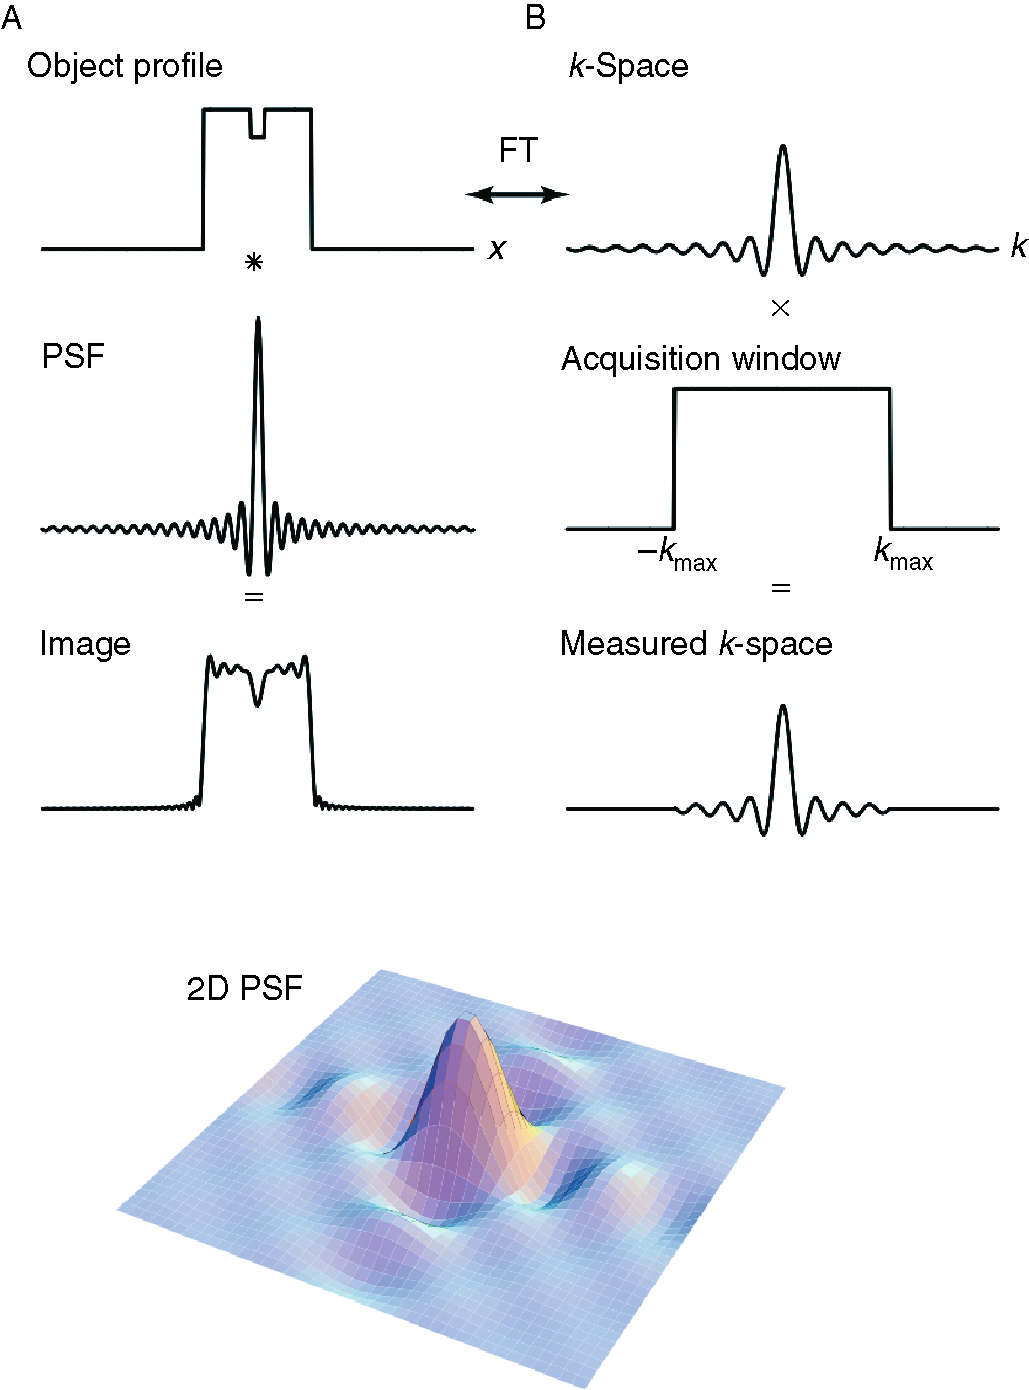
\includegraphics[width=0.68\linewidth]{imgs/kspace/psf.jpeg}
    \caption{The point-spread function. Producing a blurred image can be viewed equivalently in the image domain or in k-space. The limited extent of sampling in k-space is described by multiplying the full k-space distribution by a windowing function that removes high spatial frequencies. The resulting image is the convolution of the true image with the Fourier transform of that windowing function, the PSF. Figure adapted from \cite{buxton_fmri_2009}.}
    \label{fig:app-psf}
\end{figure}

For a rectangular window of \(N\) samples the PSF is the Dirichlet kernel,
the periodic sinc:

\begin{equation}
    \mathrm{PSF}(x) =
    \frac{\sin(\pi N x/\mathrm{FOV})}
         {N\sin(\pi x/\mathrm{FOV})}.
\end{equation}

Reading it as numerator over denominator explains its shape. Let the
pixel spacing be \(\Delta=\mathrm{FOV}/N\).

\begin{itemize}
    \item \textbf{Unit peak at \(x=0\).} Both numerator and denominator
    vanish. L'Hopital's rule gives the ratio \(\to 1\), so the centre
    pixel passes through at full weight. The kernel is normalised; no
    rescaling of \(\rho\) is required.
    \item \textbf{Zeros one pixel apart.} The numerator vanishes when
    \(\pi N x/\mathrm{FOV}=m\pi\), i.e. at
    \(x=m\,\mathrm{FOV}/N=m\Delta\). The main lobe is always exactly one
    pixel wide.
    \item \textbf{Fixed side-lobes.} The first negative side-lobe is
    approximately \(-21\%\) of the peak, or about \(-13\) dB, with a
    \(1/x\) decay. This is set purely by the rectangular window shape.
\end{itemize}

A useful consequence is that, because the zeros sit on integer pixel
offsets, an on-grid point source leaks nothing into its neighbours at the
sample points. Ringing only becomes visible at a discontinuity, where the
contributions on either side of the edge no longer cancel and the
side-lobes ring across neighbouring pixels. This is the classic
\(\approx 9\%\) Gibbs overshoot on each side of a sharp edge.

\subsection{Increasing the Matrix Does Not Fix It}

The natural reflex is to sample more of k-space, i.e. to use a bigger
box. However, a larger \(N\) only rescales the ringing; it does not
remove it.

\begin{table}
    \centering
    \begin{tabular}{ll}
        \toprule
        Quantity & Scaling with \(N\) \\
        \midrule
        Main-lobe width, physical units & \(\mathrm{FOV}/N\), shrinks as \(1/N\) \\
        Main-lobe width, pixels & 1 pixel, always \\
        First side-lobe height & \(\approx -21\%\), always \\
        Side-lobe decay & \(1/x\), always \\
        Number of side-lobes across the FOV & grows as \(N\) \\
        \bottomrule
    \end{tabular}
    \caption{Increasing the sampled matrix size improves physical resolution, but the rectangular-window PSF has the same side-lobe structure in pixel units.}
    \label{tab:app-dirichlet-scaling}
\end{table}

In pixel units the PSF shape barely changes: a larger \(N\) packs the
same ringing into a finer physical scale, giving better resolution, and
as \(N\to\infty\) the main lobe collapses towards a delta function,
recovering the ideal image. But the \(-21\%\) side-lobe is intrinsic to
the rectangular window. To actually suppress ringing, one must change the
window shape, not its size. This is apodisation.

\subsection{Apodisation: The Hamming Window}

If a hard rectangular cut is what produces the strong side-lobes, then
softening the edge of the k-space window should reduce them. This is
apodisation: weighting k-space by a function that tapers smoothly to zero
at the edges rather than truncating abruptly. Many window functions
exist; a standard choice is the Hamming window,


\begin{equation}
    w(n) =
    0.54 - 0.46\cos\left(\frac{2\pi n}{N-1}\right),
    \qquad n=0,\dots,N-1.
\end{equation}

which retains full weight near the centre, DC, and tapers to 0.08 at the
k-space edges. Because the high spatial frequencies live at those edges,
down-weighting them trades resolution for smoothness: the Fourier
transform of the Hamming window has a main lobe roughly twice as wide,
giving a blurrier image, but side-lobes suppressed from \(-13\) dB to
\(-43\) dB, giving far less ringing.

\begin{figure}
    \centering
    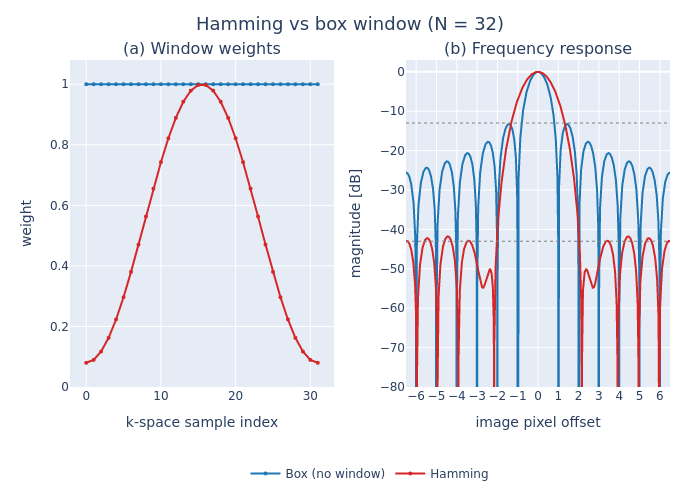
\includegraphics[width=0.72\linewidth]{imgs/kspace/hamming_window_weight.png}
    \caption{\textbf{Hamming apodisation: window weights and their point-spread response.} \textbf{(a)} K-space weighting applied before reconstruction for \(N=32\) phase-encode lines. The box window, i.e. no apodisation, weights every line equally at 1.0; the Hamming window \(0.54-0.46\cos(2\pi n/(N-1))\) tapers smoothly to 0.08 at the k-space edges, retaining full weight only near the centre. \textbf{(b)} Corresponding point-spread functions, shown as magnitude in decibels normalised to the main-lobe peak. The box window's abrupt truncation produces \(-13\) dB side-lobes that ring across neighbouring pixels; the Hamming taper suppresses these to \(-43\) dB at the cost of an approximately \(2\times\) wider main lobe, i.e. reduced spatial resolution.}
    \label{fig:app-hamming-window-weight}
\end{figure}

The effect on an actual edge is the case that matters for the phantom,
whose water--sphere boundaries are the sharpest features in the scene.
The box PSF's side-lobes fail to cancel across the step and produce the
\(\approx 9\%\) Gibbs overshoot; the Hamming PSF's far weaker side-lobes
suppress it, at the price of a softer, wider edge transition.

\begin{figure}
    \centering
    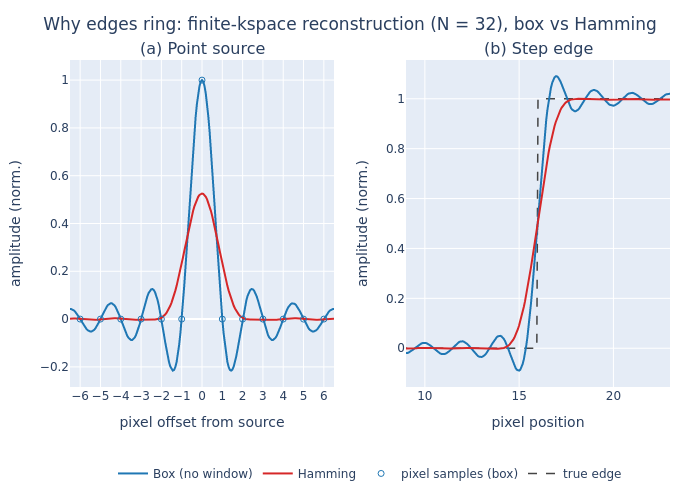
\includegraphics[width=0.74\linewidth]{imgs/kspace/hamming_ringing_psf_step_edge.png}
    \caption{\textbf{Why finite k-space sampling rings, and how Hamming apodisation suppresses it.} One-dimensional reconstruction from a finite acquisition of \(N=32\) phase-encode lines, comparing no window, or box truncation, with a Hamming window. \textbf{(a)} Point-source response: the reconstruction PSF. The box truncation yields a Dirichlet, sinc-like PSF whose zero-crossings fall exactly on integer pixel offsets. An on-grid point leaks nothing into neighbouring pixels at the sample points. The Hamming PSF has an approximately \(2\times\) wider main lobe, nonzero at \(\pm 1\) px, so it blurs adjacent pixels, and a lower peak reflecting the window's DC attenuation. \textbf{(b)} The same two PSFs convolved with a step edge. The box PSF's \(-13\) dB side-lobes fail to cancel across the discontinuity, producing Gibbs ringing with \(\approx 9\%\) overshoot on both sides. The Hamming window's \(-43\) dB side-lobes suppress this ringing, at the cost of a softer, wider edge transition. Equivalently, panel (a) is the PSF and panel (b) is that PSF convolved with an edge: the point-spread function explains the edge artefact.}
    \label{fig:app-hamming-ringing-step-edge}
\end{figure}

Two practical remarks close the loop. First, apodisation is a
reconstruction-side operation: it is an element-wise multiply applied to
the acquired k-space before the inverse FFT, costing a fraction of a
millisecond and entirely independent of the expensive Bloch simulation.
It can therefore be toggled freely without re-acquiring or re-simulating.
Second, it must not be confused with zero-padding. Padding k-space with
zeros before the FFT interpolates the image onto a finer grid but adds no
new measured frequencies, so it does not remove ringing. It only
resamples the same Dirichlet PSF more densely. Genuine suppression
requires changing the window shape, which is exactly what the phantom
library's Hamming option does, and the mechanism here is what underpins
its use against the coarse-water truncation artefact in Chapter 3.
\end{spacing}
